\section{Physikalische Grundlagen}
Die Ausführungen in diesem Abschnitt orientieren sich an \cite{manual} und an \cite{staatsex}.
\subsection{Supraleitung}
Das Auftreten von Supraleitung wird phänomenologisch dadurch beschrieben,
dass der elektrische Widerstand eines Leiters unterhalb einer bestimmten Temperatur nicht mehr
messbar ist. Für moderne Hochtemperatursupraleiter beträgt diese kritische Temperatur über 100\,K.
Die Mechanismen, die zur Supraleitung führen, sind bis heute nicht vollständig geklärt.\\
Eine Beschreibung liefert zum Beispiel die BCS-Theorie.
Hier wird die Supraleitung mit dem Auftreten von \emph{Cooper-Paaren} begründet.
Ein Cooper-Paar besteht aus zwei freien Elektronen, die über eine Entfernung von mehreren hundert Ångström
miteinander gekoppelt sind.
Die Kopplung wird verursacht durch eine Deformation (und daraus folgende Polarisation) des Kristallgitters,
wenn sich ein Elektron durch das Gitter bewegt. Ein zweites Elektron, das mit gleicher Geschwindigkeit
dem ersten Elektron folgt, wird durch die Polarisation des Gitters angezogen und bewegt sich
in einem Potentialminimum.
Die Elektronen, die einzeln als Fermionen beschrieben werden (dann gilt das Paulische Ausschlussprinzip),
werden als Cooper-Paar als einziges Boson beschrieben.
Daher können bei tiefen Temperaturen viele Cooper-Paare im gleichen Zustand existieren,
das Ausschlussprinzip gilt hier nicht.\\
Neben des verschwindenden elektrischen Widerstands zeigt ein Supraleiter das Verhalten eines idealen Diamagneten:
Ein äußeres Magnetfeld wird durch induzierte Ströme vollständig kompensiert.
Wechselt ein Material in den supraleitenden Zustand, während es sich in einem Magnetfeld befindet,
so bleibt ein konstanter Kreisstrom erhalten (Meissner-Ochsenfeld-Effekt).
Die Bohr-Sommerfeldsche Quantisierungsregel erlaubt hier allerdings nicht beliebige Stromstärken,
sondern es sind nur ganzzahlige Vielfache eines \emph{Flussquants} $\phi_0$ erlaubt.
Der Wert für $\phi_0$ beträgt
\begin{equation}
\phi_0 = 2.0678 \cdot 10^{-15}\,\text{Tm}^2 \ \, .
\end{equation}
Wird die äußere Magnetfeldstärke geändert,
so können kleine Änderungen vom Supraleiter durch induzierte Oberflächenströme kompensiert werden
(ihre Eindringtiefe wird durch die London-Gleichungen beschrieben).
Bei einer zu großen Änderung bricht die Supraleitfähigkeit allerdings zusammen,
und es stellt sich im Supraleiter ein neuer Strom ein, der das vorhandene Magnetfeld besser kompensiert.
Dann ist die Supraleitfähigkeit wieder vorhanden.\\
Der Punkt, an dem die Supraleitfähigkeit zusammenbricht, kann exakt mit einem \emph{Jo\-seph\-son-Kontakt}
eingestellt werden. Dieser Kontakt besteht aus einem wenige Nanometer dicken Isolator,
der sich im Supraleiter befindet.
Äußere Magnetfelder können in den Isolator eindringen, damit die Phasenverschiebung der Cooper-Paare,
die durch den Kontakt tunneln, beeinflussen, und so die Größe des Flussquants ändern.


\subsection{Funktionsweise des \emph{SQUID}}
Der kurzzeitige Verlust der Supraleitfähigkeit kann als Messsignal für ein äußeres Magnetfeld verwendet werden.
Man benutzt dazu einen externen Schwingkreis, der mit einem hochfrequenten Wechselstrom angeregt wird.
Die Stromamplitude ist so eingestellt, dass das resultierende Magnetfeld gerade keine Flussänderung
im Supraleiter verursacht. Wird nun das äußere Magnetfeld durch die Anwesenheit einer magnetischen Probe geändert,
so ändert sich das Magnetfeld am Supraleiter über den kritischen Wert hinaus und es kommt zu einer Änderung
des Kompensationsstroms um ein Flussquant. Dies ist mit dem kurzzeitigen
Zusammenbruch der Supraleitfähigkeit und Energieaufnahme aus dem elektromagnetischem Wechselfeld verbunden.
Der Grad der Energieaufnahme kann als Einbruch der Spannungsamplitude am Schwingkreis
gemessen werden.\\
Eine periodische Änderung des Magnetfelds führt zu einer periodischen Änderung des Signals des SQUID.
Der Zusammenhang zwischen der Signalamplitude $\Delta V$ und dem Magnetfeld $B_\text{z}$ ist folgender:
\begin{equation}
\label{eq:AtoB}
B_\text{z} = F \cdot \frac{\Delta V}{2 s_\text{i}}
\end{equation}
$F$ ist der Feld-Fluss-Koeffizient ($F$ = 9.3\,nT/$\phi_0$) und $s_\text{i}$ der Transferkoeffizient,
der die Empfindlichkeit des Messgeräts beschreibt und mit einem Widerstand $R_{\text{FB}}$ eingestellt
werden kann (siehe \autoref{tab:transfk}).
\begin{table}[H]
\caption{Zusammenhang zwischen Widerstand $R_{\text{FB}}$ und Transferkoeffizient $s_\text{i}$ (\cite{userman}).}
\begin{center}
\begin{tabular}{|c|c|c|c|c|c|c|c|c|}
\hline
$R_{\text{FB}}$ / k\text{\textOmega}	&	1	&	3	&	6	&	10	&	15	&	20	&	15	&	100	\\ \hline
$s_\text{i}$ / (mV/$\phi_0$)		&	21	&	60	&	120	&	195	&	290	&	380	&	950	&	1900	\\ \hline
\end{tabular}
\end{center}
\label{tab:transfk}
\end{table}

\subsection{Magnetfeld einer Leiterschleife}
Die magnetische Flussdichte $\difd \vec{B}$ am Ort $\vec{r}$ eines mit dem Strom $I$ durchflossenen
Leiters mit Länge $\difd \vec{l}$ 
am Ort $\vec{r}'$ lässt sich mit Hilfe des \emph{Biot-Savart}-Gesetzes bestimmen:
\begin{equation}
  \label{eq:biotsavart}
  \difd \vec{B}(\vec{r}) = \frac{\mu_0 \cdot I}{4 \pi} \cdot \difd \vec{l} \times \frac{\vec{r} - \vec{r}'}{\abs{\vec{r} - \vec{r}'}^3}
\end{equation} 

\begin{figure}[H]
\begin{center}
  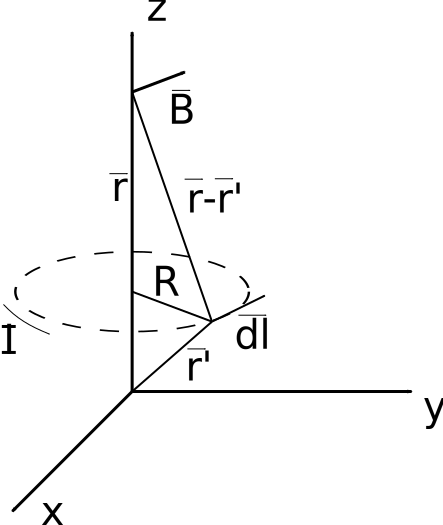
\includegraphics[width=0.3\textwidth]{../img/circloop.pdf}
  \caption{Kreisförmige Leiterschleife mit Radius $R$, parallel zur $x$-$y$-Ebene.}
  \label{img:circloop}
\end{center}
\end{figure}

Es wird eine kreisförmige Leiterschleife parallel zu der $x$-$y$-Ebene
mit dem Radius $R$ betrachtet (\autoref{img:circloop}) \cite{dem2}.
Da die Komponente
\begin{equation}
\difd B_\perp = \difd B \cdot \sin \alpha
\end{equation}
senkrecht zur $z-$Achse bei der Integration über $\difd l$ verschwindet 
(Rotationssymmetrie), bleibt nur die parallele Komponente
\begin{equation}
\difd B_\parallel = \difd B \cdot \cos \alpha
\end{equation}
zu betrachten. Wie in 
\autoref{img:bvector} zu erkennen ist, gilt
\begin{equation}
\label{eq:absdif}
  \abs{\difd \vec{l} \times \left( \vec{r} - \vec{r}' \right)} = \abs{\vec{r} - \vec{r}'} \cdot \difd l \cdot \underbrace{\sin \varphi}_{= 1} 
  = \abs{\vec{r} - \vec{r}'} \cdot \difd l = \frac{R}{\cos \alpha} \cdot \difd l
\end{equation}
\begin{figure}[H]
\begin{center}
  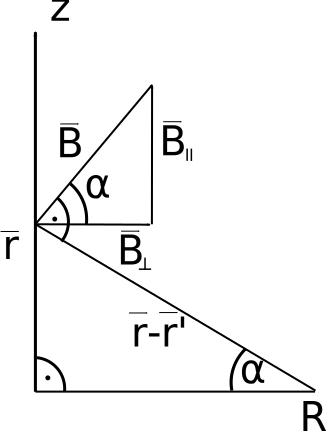
\includegraphics[width=0.3\textwidth]{../img/bvector.pdf}
  \caption{Komponenten des $\vec{B}$-Vektors und Dreieck zwischen $R$, $\vec{r}-\vec{r}'$ und $\vec{r}$.}
  \label{img:bvector}
\end{center}
\end{figure}
Es folgt für $B_\parallel$:
\begin{equation}
\begin{split}
  \label{eq:bparallel}
    B_\parallel &= \int \difd B_\parallel = \int \difd B \cdot \cos \alpha \\
  &\refeq{eq:biotsavart} \frac{\mu_0 \cdot I}{4 \pi} \cdot \oint \frac{\abs{\difd \vec{l} \times \left( \vec{r} - \vec{r}' \right)}}{\abs{\vec{r} - \vec{r}'}^3} \cdot \cos \alpha \\
  &\refeq{eq:absdif} \frac{\mu_0 \cdot I}{4 \pi} \cdot \frac{R}{\abs{\vec{r} - \vec{r}'}^3} \cdot \oint \difd s = \frac{\mu_0 \cdot I}{2} \cdot \frac{R^2}{\abs{\vec{r} - \vec{r}'}^3}
\end{split}
\end{equation}
Mit $\abs{\vec{r} - \vec{r}'}^2 = R^2 + (z-z')^2$ folgt damit für die magnetische Flussdichte $\vec{B}(z, z')$
\begin{equation}
  \label{eq:Bz:biotsavart}
  \vec{B}(z, z') = B_\parallel \cdot \hat{e}_z \refeq{eq:bparallel} \frac{\mu_0 \cdot I}{2} \cdot \frac{R^2}{ \left( R^2 + (z-z')^2 \right)^{3/2}} \cdot \hat{e}_z
\end{equation}

Dieser Zusammenhang wird in der Auswertung mit den Messwerten verglichen.
